\problemname{Dimensional Debugging}

%\illustration{0.3}{image.jpg}{Caption of the illustration (optional). CC BY-NC 2.0 by X on Y}
% Source: URL to image.

% optionally define variables/limits for this problem
\newcommand{\maxk}{10}
\newcommand{\maxn}{1000}
\newcommand{\maxc}{10^9}

After struggling with this \emph{one} problem for \emph{days}, you have had
enough! You are determined to find the bug in your algorithm once and for all!
To do so, you will start all over. From scratch. At least you are sure you know
the correct answer in the most trivial case: the answer in $(0,0, \dots, 0)$
is $0$.

You will re-solve the problem, which takes $k$ parameters,
using $n$ simpler but slower algorithms.
Each algorithm has two bounds for every parameter $i$ ($L_i$ and $H_i$).
An algorithm is only fast enough to run on inputs
$(x_1, \dots, x_k)$ where $x_i \leq H_i$ for all parameters $i$.
You are confident the implementation of an algorithm
is correct if you can verify its correctness at least once on an input
$(x_1, \dots, x_k)$ where $x_i \geq L_i$ for all parameters $i$.
To do so, you will need another algorithm
that you already proved to be correct and can handle such large inputs,
or your knowledge of the answer for $(0,0, \dots, 0)$.

Given a list of algorithms and their bounds,
find the number of algorithms you are sure are correctly implemented.

As an example, consider the first sample case shown in
Figure~\ref{fig:debugging} on the left.
The first algorithm (red, bottom left) can be used to verify the
correctness of the second (yellow, top left) and third (blue, bottom right) algorithms. No algorithm
can be used to verify the correctness of the fourth algorithm (grey, top right).

\begin{figure}[!h]
\centering

\hfill%
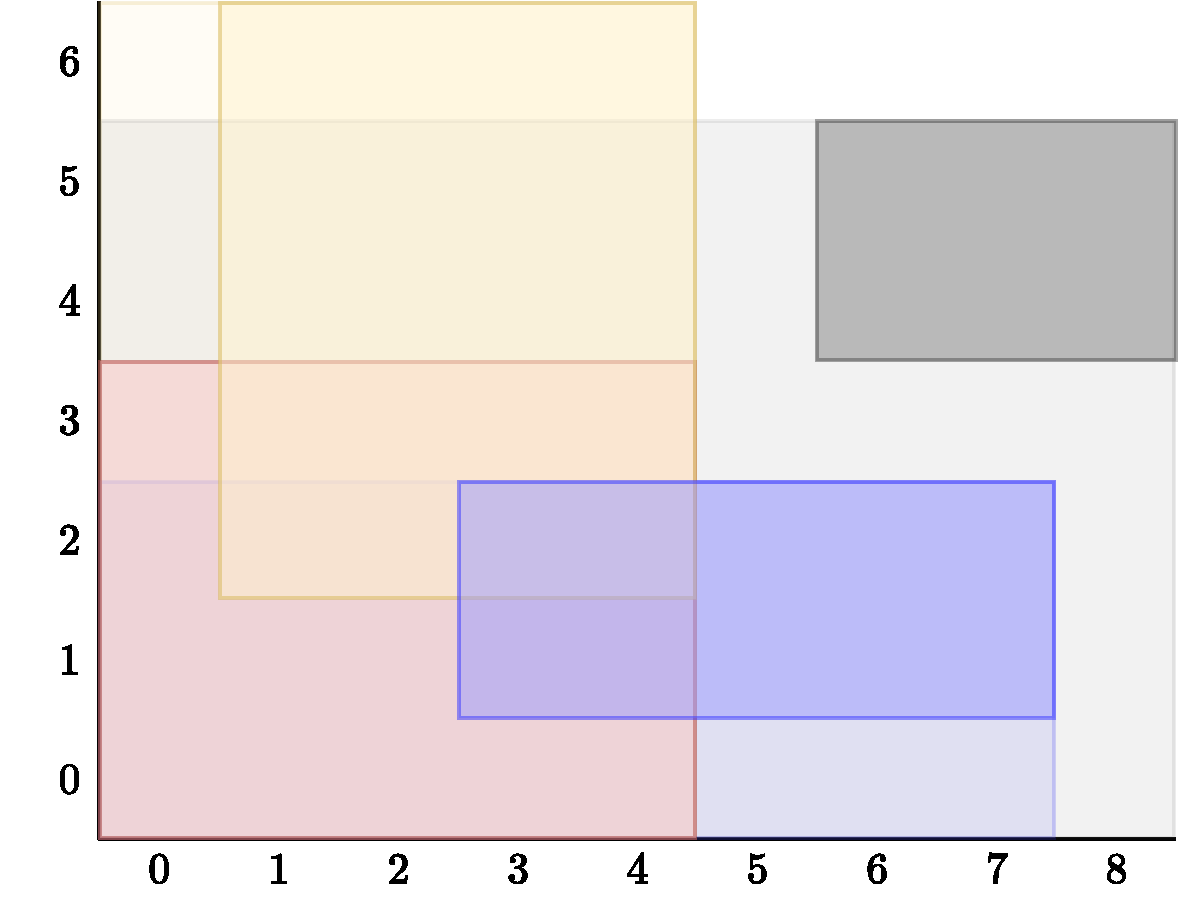
\includegraphics[width=0.35\textwidth]{sample1}%
\hfill%
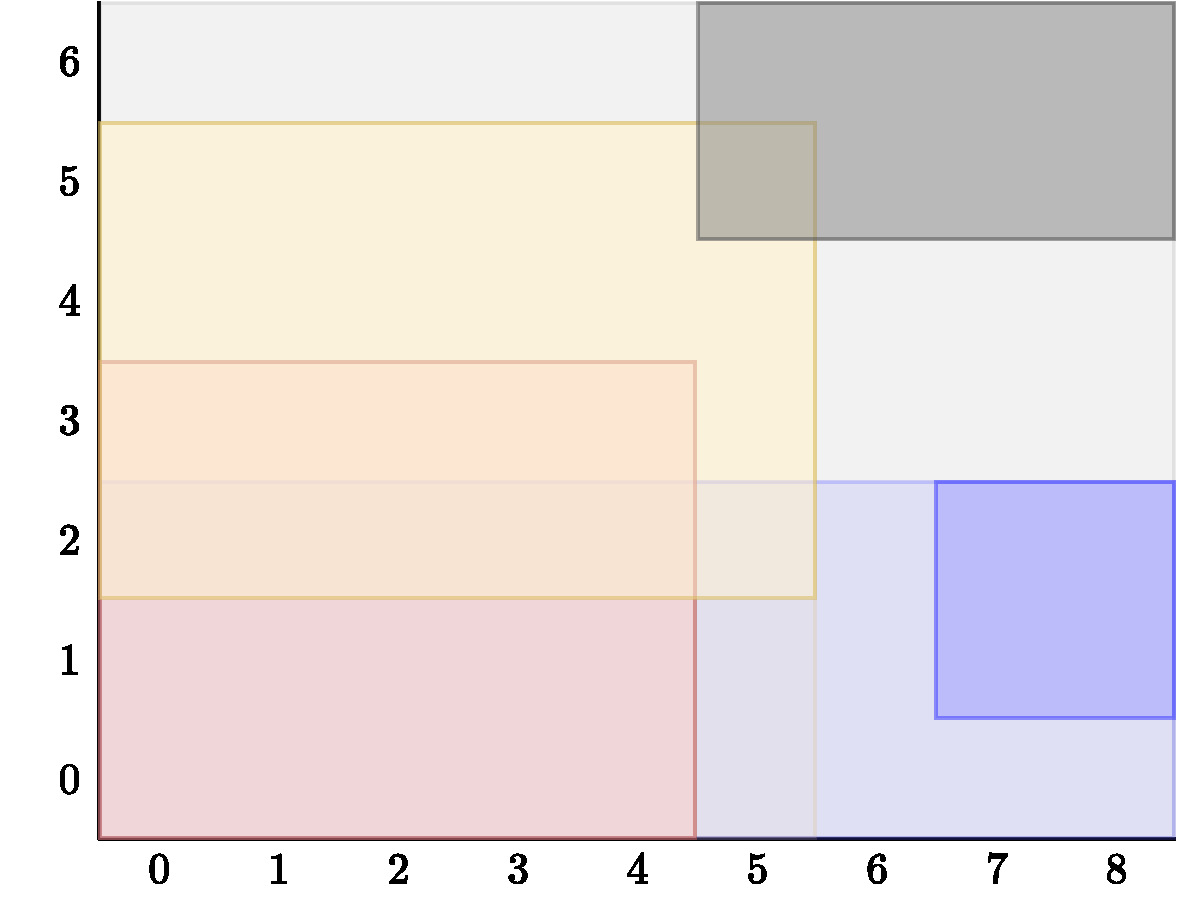
\includegraphics[width=0.35\textwidth]{sample2}%
\hfill%
\hfill% One extra hfill actually makes them centered, don't ask me why... https://tex.stackexchange.com/a/349356

\caption{
    \centering
    The algorithms to be tested in samples 1 and 2, respectively.
    The boxes indicate the parameters where an algorithm must be tested,
    while the lighter background indicates the region
    where an algorithm can be used to verify other algorithms.
}
\label{fig:debugging}
\end{figure}

\vspace{-1em}

\begin{Input}
  The input consists of:
  \begin{itemize}
    \item One line with two integers $n$ and $k$ ($1\leq n\leq \maxn$, $1\leq k\leq \maxk$),
          the number of algorithms to test and the number of parameters.
    \item Then follow $n$ pairs of lines:
          \begin{itemize}
            \item One line with $k$ integers
                  $L_i, \dots, L_k$ ($0\leq L_i \leq \maxc$ for all $i$).
            \item One line with $k$ integers
                  $H_1, \dots, H_k$ ($0\leq H_i \leq \maxc$ for all $i$).
            \end{itemize}
          It is guaranteed that $L_i \leq H_i$ for all $1 \leq i\leq k$.
  \end{itemize}
\end{Input}

\begin{Output}
    Output the number of algorithms of which you can verify the correctness.
\end{Output}
